\documentclass{beamer}
\usepackage[utf8]{inputenc}
\usepackage[T1]{fontenc}
\usepackage{lmodern}
\usepackage{tikz}
\usetikzlibrary{math}
\usetikzlibrary{snakes}
\usetikzlibrary{decorations.pathreplacing}
\usepackage[absolute,overlay]{textpos}
\usepackage{booktabs}
\usepackage{ulem}
\usepackage{array}


\title{Abschlusspräsentation}
\author{Projektgruppe FastSense}
\date{11. März 2021}

\usecolortheme{seahorse}
\definecolor{dark}{rgb}{0, 0.1, 0.3}
\definecolor{light}{rgb}{0.9, 0.933, 1}
\definecolor{hw}{rgb}{0.8, 1, 0.9}
\definecolor{red}{rgb}{1, 0, 0}
\definecolor{yellow}{rgb}{1, 1, 0}
\definecolor{green}{rgb}{0, 1, 0}
\definecolor{cyan}{rgb}{0, 1, 1}
\definecolor{blue}{rgb}{0, 0, 1}
\definecolor{magenta}{rgb}{1, 0, 1}
\definecolor{grey}{rgb}{0.8, 0.8, 0.8}
\setbeamercolor{normal text}{fg=black}
\setbeamercolor{structure}{fg=dark}
\setbeamercolor{footline}{fg=black}
\setbeamercolor{frametitle}{fg=light,bg=dark}
\setbeamertemplate{itemize items}[circle]
\beamertemplatenavigationsymbolsempty
\addtobeamertemplate{navigation symbols}{}{
    \usebeamerfont{footline}
    \usebeamercolor[fg]{footline}
    {\footnotesize \insertframenumber\\\vspace{0.15cm}}
}
\setbeamertemplate{title page}{
\insertauthor\\
\vspace{0.5cm}
\begin{LARGE}\textbf{\inserttitle}\end{LARGE}\\
\vspace{0.5cm}
\insertdate
}

\begin{document}

{\setbeamertemplate{navigation symbols}{}
\begin{frame}
\titlepage
\end{frame}}

\section{Motivation}
\begin{frame}{\secname}
\begin{textblock*}{12cm}(1cm,2cm)
\begin{itemize}
\item{TODO}
\end{itemize}
\end{textblock*}
\end{frame}

\section{Problematik}
\begin{frame}{\secname}
TODO
\end{frame}

\section{Ziele}
\begin{frame}{\secname}
TODO
\end{frame}

\section{MS1: Trail Detection}
\begin{frame}{\secname}
TODO    
\end{frame}

\section{SLAM-Box}
\begin{frame}{\secname}
TODO
\end{frame}

\section{TSDF}
\begin{frame}{\secname}
\begin{center}
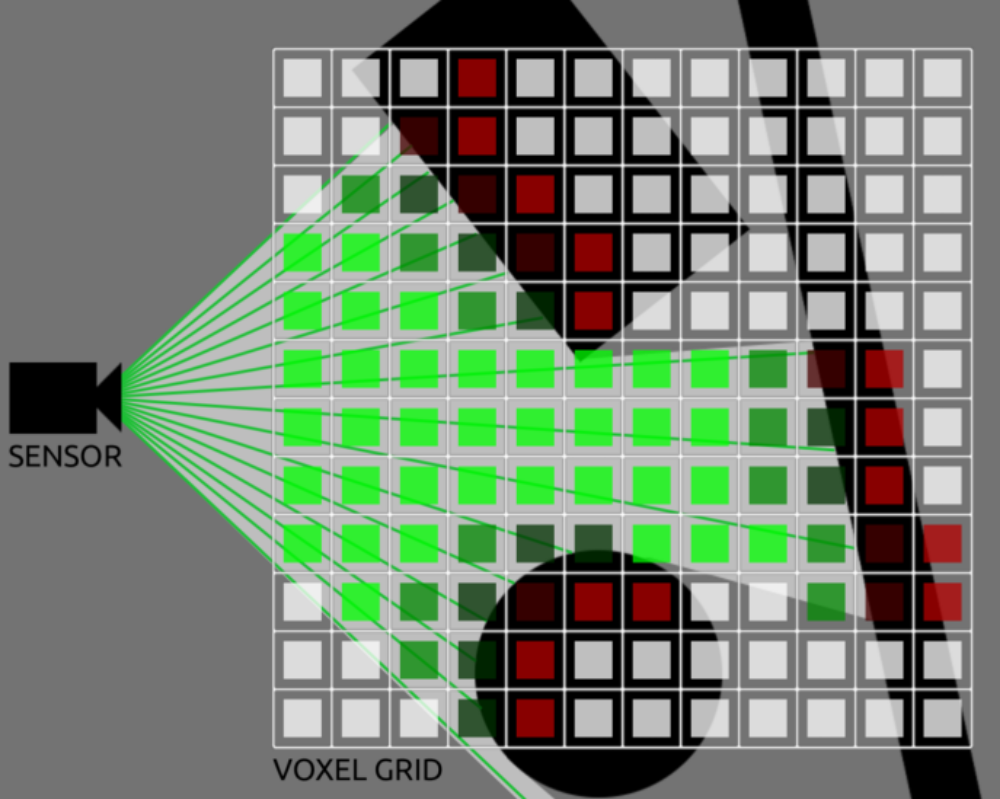
\includegraphics[width=5cm]{images/TSDF_Gen_new.png}
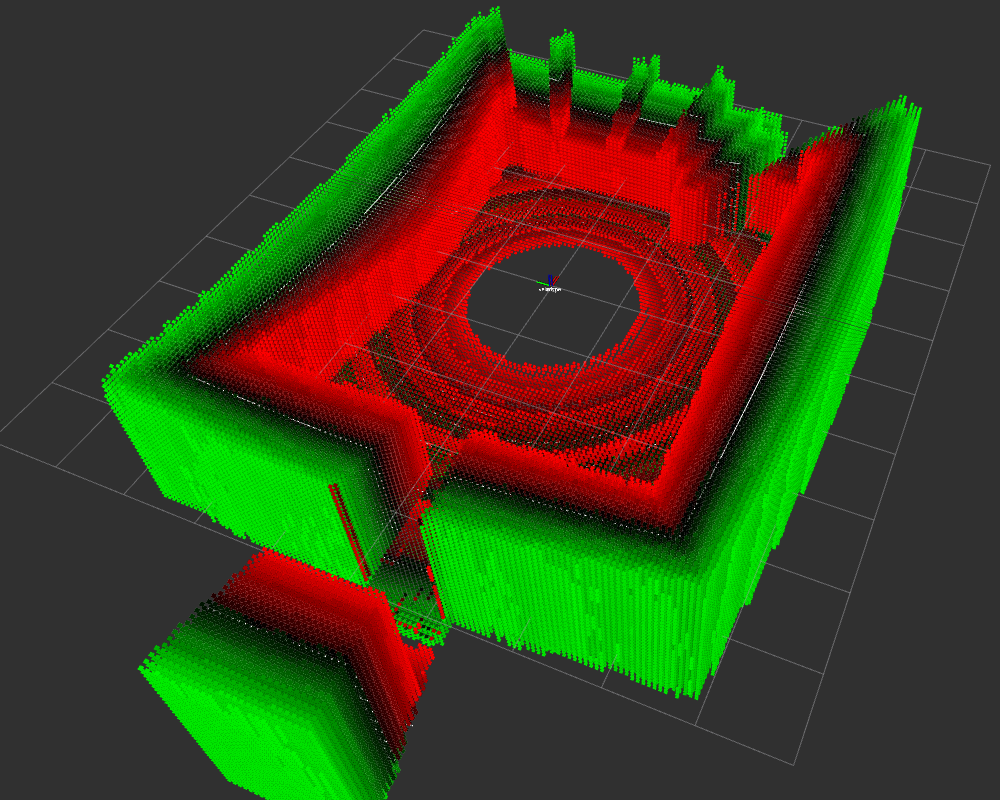
\includegraphics[width=5cm]{images/TSDF_3D.png}
\end{center}
\end{frame}

\section{Point-to-TSDF Registrierung}
\begin{frame}{\secname}
\begin{center}
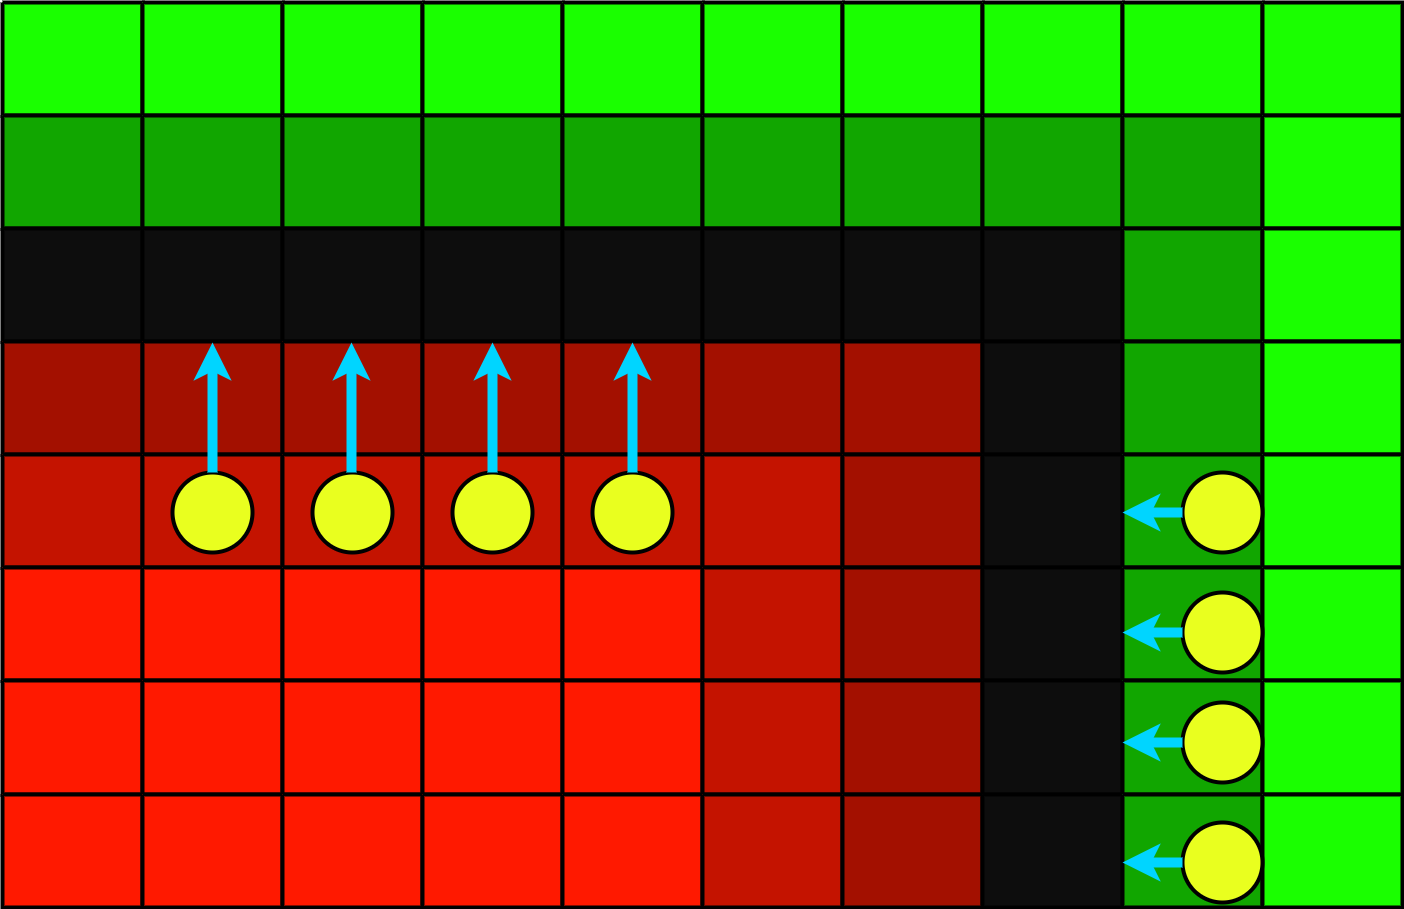
\includegraphics[width=5cm]{images/Reg_Gradient.png}
\end{center}
\end{frame}

\section{Hardware Architektur}
\begin{frame}{\secname}
TODO
\end{frame}

\section{Vorgehen}
\begin{frame}{\secname}
TODO    
\end{frame}

\section{Aufbau}
\begin{frame}{\secname}
TODO    
\end{frame}

\section{Evaluation}
\subsection{Performance}
\begin{frame}{\secname: \subsecname}
TODO
\end{frame}

\subsection{Power Consumption}
\begin{frame}{\secname: \subsecname}
TODO
\end{frame}

\subsection{Accuracy}
\begin{frame}{\secname: \subsecname}
TODO
\end{frame}

\section{Fazit}
\begin{frame}{\secname}
TODO    
\end{frame}

\section{Ausblick}
\begin{frame}{\secname}
TODO
\end{frame}

\end{document}
